\subsection{The Braess Network}

As a croncrete network we introduce the Braess Network as described by \citet{Murchland1970} in \cref{fig:braess-network}.

\begin{figure}[!ht]
    \centering
    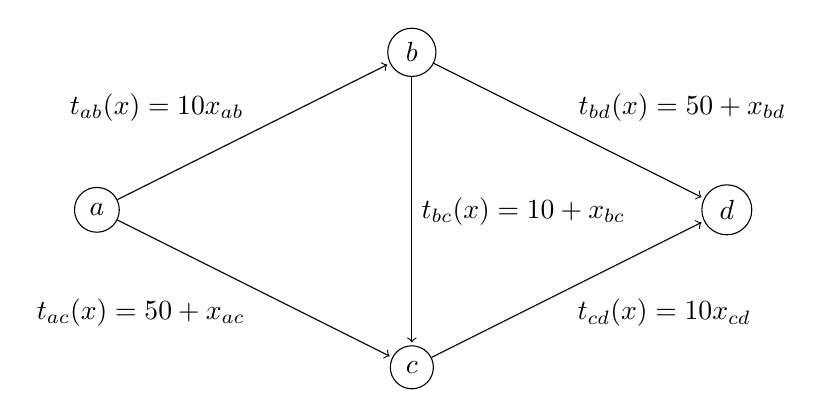
\begin{tikzpicture}[vertex/.style={circle, draw}]
        \node[style=vertex] (a) at (-4, 0)  {$a$};
        \node[style=vertex] (b) at (0, 2)  {$b$};
        \node[style=vertex] (c) at (0, -2) {$c$};
        \node[style=vertex] (d) at (4, 0)  {$d$};
        
        \draw[every loop]
            (a) edge node[above left] {$t_{ab}(x)=10 x_{ab}$} (b)
            (a) edge node[below left] {$t_{ac}(x)=50 + x_{ac}$} (c)
            (b) edge node[above right] {$t_{bd}(x)=50 + x_{bd}$} (d)
            (c) edge node[below right] {$t_{cd}(x)=10 x_{cd}$} (d)
            (b) edge node[right] {$t_{bc}(x)=10+x_{bc}$} (c)
        ;
    \end{tikzpicture}
    \caption{The Braess network. Each link is labeled with the link cost function.}
    \label{fig:braess-network}
\end{figure}

On this network there is only one origin-destination pair: $(a, d)$.
Let $q=6$ denote the travel demand from $a$ to $d$.
Further, we assume that the road network has sufficient capacity for all vehicles.
In particular, we may take capacity equal to $q$ for each link. 
There are three paths between $a$ and $d$ on this network: $(a, b, d)$, $(a,c,d)$, and $(a, b, c, d)$.
We will refer to these three paths as \textit{upper}, \textit{lower}, and \textit{zig-zag} paths respectively.

\citet{Murchland1970} states the equilibrium is achieved when each of the three paths is used by two vehicles each.
Immediately we see that such a path flow is demand-feasible since the path flows sum to equal the demand.
To convince ourselves that such a path flow is indeed at equilibrium, we can apply Wardrop's first principle directly: all used paths should have equal travel cost.
First, let us compute the corresponding link flow.
We could construct the link-path incidence matrix, but for this small example it is easier to simply enumerate in \cref{tab:braess:equilibrium-costs}.
The link cost is computed by applying the link cost function associated with each link in \cref{fig:braess-network}.

\begin{table}[!ht]
\centering
\caption{Link flow and link costs}\label{tab:braess:equilibrium-costs}
\begin{tabular}{@{}l|lll|ll@{}}
\toprule
Link & Upper & Lower & Zig-zag & Link flow & Link cost \\ \midrule
ab   & 2     & 0     & 2       & 4         & 40        \\
bd   & 2     & 0     & 0       & 2         & 52        \\
ac   & 0     & 2     & 0       & 2         & 52        \\
cd   & 0     & 2     & 2       & 4         & 40        \\
bc   & 0     & 0     & 2       & 2         & 12        \\ \bottomrule
\end{tabular}
\end{table}

We can compute the path costs by simply adding up the costs on each link of the path.
The upper path is composed of ab and bd, the lower by ac and cd, and the zig-zag by ab, bc, and cd.
The path costs are therefore $40+52=92$ for the upper path, $52+40=92$ for the lower path, and $40+12+40=92$ for the zig-zag path.
We observe that all paths that are used have equal cost.
Therefore Wardrop's first condition is met and this link flow is an equilibrium.

Alternatively we use this example to understand why Wardrop's first condition is equivalent to the condition that no driver has a less costly alternative route.
When all paths between their origin and destination cost the same, the driver had no incentive to switch routes.

Additionally, we can use the VI path flow formulation at this equilibrium and show that the following holds for all feasible path flows.

\begin{align*}
    \mathbf{T}(\mathbf{f}^*)\mathbf{f} - \mathbf{T}(\mathbf{f}^*)\mathbf{f}^* &\geq 0\\
    92\cdot f_{\text{upper}} + 92\cdot f_{\text{lower}} + 92 \cdot f_{\text{zig-zag}} - (92\cdot 2 + 92\cdot 2 + 92\cdot 2) &\geq 0\\
    f_{\text{upper}} + f_{\text{lower}} + f_{\text{zig-zag}} &\geq 6
\end{align*}

Recall that a path flow is feasible if the total volume over paths between and origin-destination pair is equal to the demand between that pair.
Therefore, $f_{\text{upper}} + f_{\text{lower}} + f_{\text{zig-zag}}=6$ for all feasible path flows and the inequality holds.\\


This particular network is notable because its equilibrium traffic flow is not its most efficient traffic assignment, giving rise to what is known as the ``Braess Paradox''.
Consider instead the demand-feasible path flow which puts three vehicles each on the upper and lower paths and none on the zig-zag path.
The link costs for this path flow are given in \cref{tab:braess:optimal-costs}.

\begin{table}[!ht]
\centering
\caption{Link flow and link costs}\label{tab:braess:optimal-costs}
\begin{tabular}{@{}l|lll|ll@{}}
\toprule
Link & Upper & Lower & Zig-zag & Link flow & Link cost \\ \midrule
ab   & 3     & 0     & 0       & 3         & 30        \\
bd   & 3     & 0     & 0       & 3         & 53        \\
ac   & 0     & 3     & 0       & 3         & 53        \\
cd   & 0     & 3     & 0       & 3         & 30        \\
bc   & 0     & 0     & 0       & 0         & 10        \\ \bottomrule
\end{tabular}
\end{table}

With this path flow, the travel costs on each of the used paths is 83.
This is less than the cost of the paths at equilibrium, meaning that this is globally more efficient.
However, this flow pattern is not an equilibrium because the unused zig-zag path has cost equal to 70 ($=30+10+30$), less than the cost of the used paths.
As a result, a single driver on the upper or lower path would be able to switch to the zig-zag path and save time.
This fact contradicts Wardrop's first condition.

As a VI in the path flow formulation we may find a path flow which does not satisfy the inequality.

\begin{align*}
    \mathbf{T}(\mathbf{f}^*)\mathbf{f} - \mathbf{T}(\mathbf{f}^*)\mathbf{f}^* &\geq 0\\
    83\cdot f_{\text{upper}} + 83\cdot f_{\text{lower}} + 70 \cdot f_{\text{zig-zag}} - (83\cdot 3 + 83\cdot 3 + 70\cdot 0) &\geq 0\\
    83\cdot f_{\text{upper}} + 83\cdot f_{\text{lower}} + 70 \cdot f_{\text{zig-zag}} \geq 83\cdot 6 
\end{align*}

In particular take $f_{\text{zig-zag}}=6$ (and no flow on either of the other two paths). Substituting this path flow into the inequality yields $70\cdot 6 \geq 83 \cdot 6$ which is false.
